\documentclass[10pt]{beamer}

% Handout Generation {{{

% \documentclass[10pt,handout]{beamer}
% \usepackage{pgfpages}
% \pgfpagesuselayout{4 on 1}[a4paper, landscape, border shrink=5mm]
% \pgfpageslogicalpageoptions{1}{border code=\pgfusepath{stroke}}
% \pgfpageslogicalpageoptions{2}{border code=\pgfusepath{stroke}}
% \pgfpageslogicalpageoptions{3}{border code=\pgfusepath{stroke}}
% \pgfpageslogicalpageoptions{4}{border code=\pgfusepath{stroke}}

% Packages {{{1

\usepackage{graphicx}
\usepackage{xcolor}
\usepackage{tikz}

\definecolor{KTHBlue}{HTML}{003C9E}

% Theming {{{1
\usetheme[progressbar=foot]{metropolis}

\setbeamercolor{normal text}{%
	fg=black!90,
	bg=black!2
}
\setbeamercolor{alerted text}{%
	fg=KTHBlue!80,
	bg=black!2
}
\setbeamercolor{palette primary}{%
	use=normal text,
	fg=normal text.bg,
	bg=KTHBlue
}
\setbeamercolor{progress bar in head/foot}{fg=KTHBlue, bg=KTHBlue!10}
\setbeamercolor{progress bar in section page}{fg=KTHBlue, bg=KTHBlue!10}
\setbeamercolor{title separator}{fg=KTHBlue}

% Title Page {{{1

\title{Coding Best Practices \& Tools}
\subtitle{Towards painless maintable programming for researchers}
\date{MWL Lunch Seminar -- June 2016}
\author{L. \textsc{Manzari} -- M. \textsc{Gaborit}}
\institute{}
\titlegraphic{\hfill\includegraphics[height=1.5cm]{logo}}

% Graphics {{{1

\newcommand\fileimage[1]{%
	\draw (#1) -- ++(2,0) -- ++(0,2.5) -- ++(-1.5,0) -- ++(-.5,-.5) -- cycle;
}


% }}}
\begin{document}

% Title and TOC {{{1
\maketitle

\begin{frame}{Contents}
	\setbeamertemplate{section in toc}[sections numbered]
	\tableofcontents[hideallsubsections]
\end{frame}

\section{Better coding practices ?} % {{{1

\begin{frame}{From research to industry}
	TODO
\end{frame}

\section{Editors \& IDE} % {{{1

\begin{frame}{Filetypes in research} % {{{2

	\begin{center}
		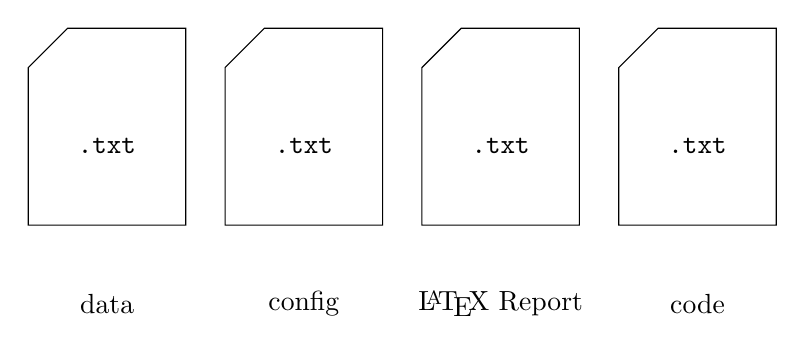
\begin{tikzpicture}
			\foreach \type [count=\i] in {data,config,{\LaTeX{} Report},code}{
				\fileimage{2.5*\i,0};
				\node (tmp) at (2.5*\i+1,-1) {\type};
				\node (tmp) at (2.5*\i+1,1) {\textbf{\texttt{.txt}} };
				\pause{}
			}
		\end{tikzpicture}
		\pause{}

		\Large
		All are \alert{text files}...
		\pause{}

		$\Rightarrow$ Need a good editor !
	\end{center}
\end{frame}

\begin{frame}{What is a good editor ?} % {{{2
	\begin{itemize}
		\item Focuses on editing and file content
		\item Eases writing (code completion, syntax highlighting, \textit{etc.})
		\item Syntaxic checking
		\item Customizable \& Extensible
	\end{itemize}

	\pause{}
	\begin{block}{Plugins done right} % {{{2
		Always prefer a simple editor and a few, carefuly chosen, plugins to a all-doing
		overcomplicated software.
	\end{block}

	\pause
	\begin{block}{Plugins done right (UNIX Version)}
		It does only one thing but it does it perfectly.
	\end{block}
\end{frame}

\begin{frame}[t]{Editors : VIm} % {{{2
	\only<1>{
		\begin{block}{What people think it is...}
			\begin{center}
			\includegraphics[width=.9\textwidth]{images/vim/people_think.png}
		\end{center}
		\end{block}
	}
	\only<2>{
		\begin{block}{What it does actually look like}
			\begin{center}
			\includegraphics[width=.9\textwidth]{images/vim/actual.png}
			\end{center}
		\end{block}
	}
	\only<3>{
		\begin{block}{Characteristics}
			\begin{itemize}
				\item Command line or GUI
				\item Modal (one mode per class of action : edition, displacement, selection, etc...)
				\item Based on shortcuts and commands
				\item Fully customizable through plugin or embedded language
				\item Painless integration with any standard UNIX toolchain
			\end{itemize}
		\end{block}
		\begin{block}{Where to start}
			\begin{itemize}
				\item \url{http://vim-adventures.com/}
				\item \texttt{\$ vimtutor}
				\item \url{http://vimcasts.org/}
				\item \url{https://vimebook.com/en}
			\end{itemize}
		\end{block}
	}
\end{frame}

\begin{frame}[t]{Editor : Emacs} % {{{2
 	TODO
\end{frame}

\begin{frame}[t]{Editor : SublimeText, Atom, Light Table} % {{{2
	TODO
\end{frame}
% }}}

\section{Versionning for fun and profit} % {{{1

\begin{frame}[t]{Contribution to a research code} % {{{2
	\begin{center}
		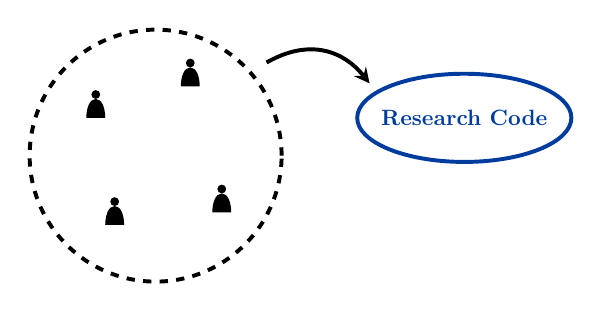
\begin{tikzpicture}[>=stealth, scale=.8, transform shape]
			% central node
			\node[KTHBlue] (researchcode) at (0,0) {\textbf{Research Code}};
			\draw[KTHBlue, line width=.5mm] (0,0) ellipse (1.7 and .7);

			% team
			\newcommand\teammember[1]{%
				\fill[black] (#1) -- ++(.3,0) .. controls ++(0,.15) and ++(.1,0) .. ++(-.15,.3) .. controls ++(-.1,0) and ++(0,.15) .. (#1);
				\fill[black] (#1) ++(.15,.37) circle (.07);
			}

			\foreach \x/\y in {-6/0, -4.5/.5, -4/-1.5, -5.7/-1.7}{
				\teammember{\x,\y};
			}
			\draw[dashed, line width=.5mm] (-4.9,-.6) circle (2);
			\draw[->, line width=.5mm] (-4.9,-.6) ++(40:2.3) .. controls ++(.7,.4) and ++(-.4,.5) ..  (160:1.6);

		\end{tikzpicture}
	\end{center}
\end{frame}

% }}}

\section{Documentation is not a myth} % {{{1

\section{What's next ?} % {{{1


\begin{frame}[standout] % Thank you {{{1
	Thank you !\\
	\vspace{0.05\textwidth}
	Questions ?\\
	\vspace{0.25\textwidth}
	\scriptsize{\texttt{manzari@kth.se}} --- \scriptsize{\texttt{gaborit@kth.se}}\\
\end{frame}

%}}}
\end{document}
